\chapter{Results}
In this chapter we evaluate the functionality of our approach \todo{evaluate the learning performance of the resulting library?}. In the first section\XX{,} we attempt to optimize \todo{describe the process of the optimization of?} the neural network parameters, in order to achieve the best performance. In the next sections\XX{,} we optimize the parameters of the algorithm and evaluate its performance. For the purposes of evaluation, we have decided to use fixed four shape descriptors, namely the square, circle, triangle and water drop shape descriptors throughout this chapter. If the number of shape descriptors changes, it is possible that the optimal value of same parameters might change as well. \todo{same method can be applied to re-establish the modified optimal parameters?} 

\section{Neural networks performance}
For the correct functionality of the algorithm, it is required that the network is able to recognize the shapes. There are numerous parameters for the neural networks, like the training algorithm choice, architecture and activation function. Because it is not feasible to test every combination of the parameters, we have tested the influence of only a several of these parameters.

\subsection{Setup}
In order to test some of the network parameters, we have fixed the configuration parameters that were not tested with the following setup:
\begin{description}
\item [Network architecture] The networks have a layered structure, with two hidden layers. However, we have tested the influence of different sizes of the layers.
\item [Training algorithm] The networks are trained using resilient back-propagation algorithm from the FANN library.
\item [Activation function] The neurons of the network use the Elliot activation function, a faster version of the sigmoid activation function.
\item [Shape descriptors] We have used four basic shapes descriptors: square, circle, triangle and a water drop throughout the the whole chapter. 
\item [Data] The training data and the test data were generated by the developed generator. The training data consisted of 150 000 images, where each shape had the same amount of examples, and 50 000 images of random data. The test data consisted of 40 000 images of examples of shapes, and 20 000 images of random data.
\end{description}

\subsection{Tested parameters}
We have tested the combinations o the following parameters:
\begin{description}
\item [Layer size] We have tried several values for both layers. For the first hidden layer, we have tried 100, 200 and 300 neurons, and for the second hidden layer 10, 20 and 30 neurons. These values were chosen heuristically.
\item [The value of MSE] We have trained the networks at different levels of precision, with the target MSE values of 0.1, 0.07, 0.04 and 0.01.
\item [Algorithm settings] The neural networks were trained for different combinations of algorithm settings, with embeddings and composition turned off and on.
\end{description}
We trained the networks with all the combinations of the parameters above, which gave us 3*3*4*4 = 150 trained neural networks to evaluate.

\subsection{Evaluation}
The networks were evaluated in the following scenario. For each of the combinations of embeddings and composition being turned on or off, the dataset of 1000 images was generated, with the same amount of examples for each shape. Then, the network was assigned a score computed as a sum of scores over all examples. Score per example was assigned by the following rules, in order to mimic the actual usage in the algorithm, where we consider only the maximum output:

\begin{description}
\item [1] If the maximum of the outputs of the network is in the corresponding output neuron of the shape that is in the example, which means, that the network classified the shape correctly.
\item [2] If the maximum of in the correct output neuron and is higher than 0.7. 
\item [-1] If the maximum is in the wrong output neuron which corresponds to the different shape than the one in the image, and the value is higher than 0.7.
\item [0] Otherwise.
\end{description}

These rules \label{rules} mimic the usage of the network in the algorithm, where only maximum values above 0.7 are considered. The value 0.7 was chosen because the scores of the networks differ more with a numbers closer to 1, and the plots are more clear. From the rules follows, that each network could achieve from -1000 to 2000 score points on a dataset of 1000 samples.

\subsection{Results}
\cref{fig:simples}, \cref{fig:embed}, \cref{fig:comp} and \cref{fig:cmb} show the score of the networks achieved on different evaluation datasets. The datasets contain 1000 samples each, but differ in the techniques used in the images. The first dataset contains only simple shapes, without embeddings or conglomeration, the second contains embeddings only, the third composition only, and finally the fourth contains both embeddings and composition combined.

\todo{check if caption reference is ok}
\begin{figure}
\centering
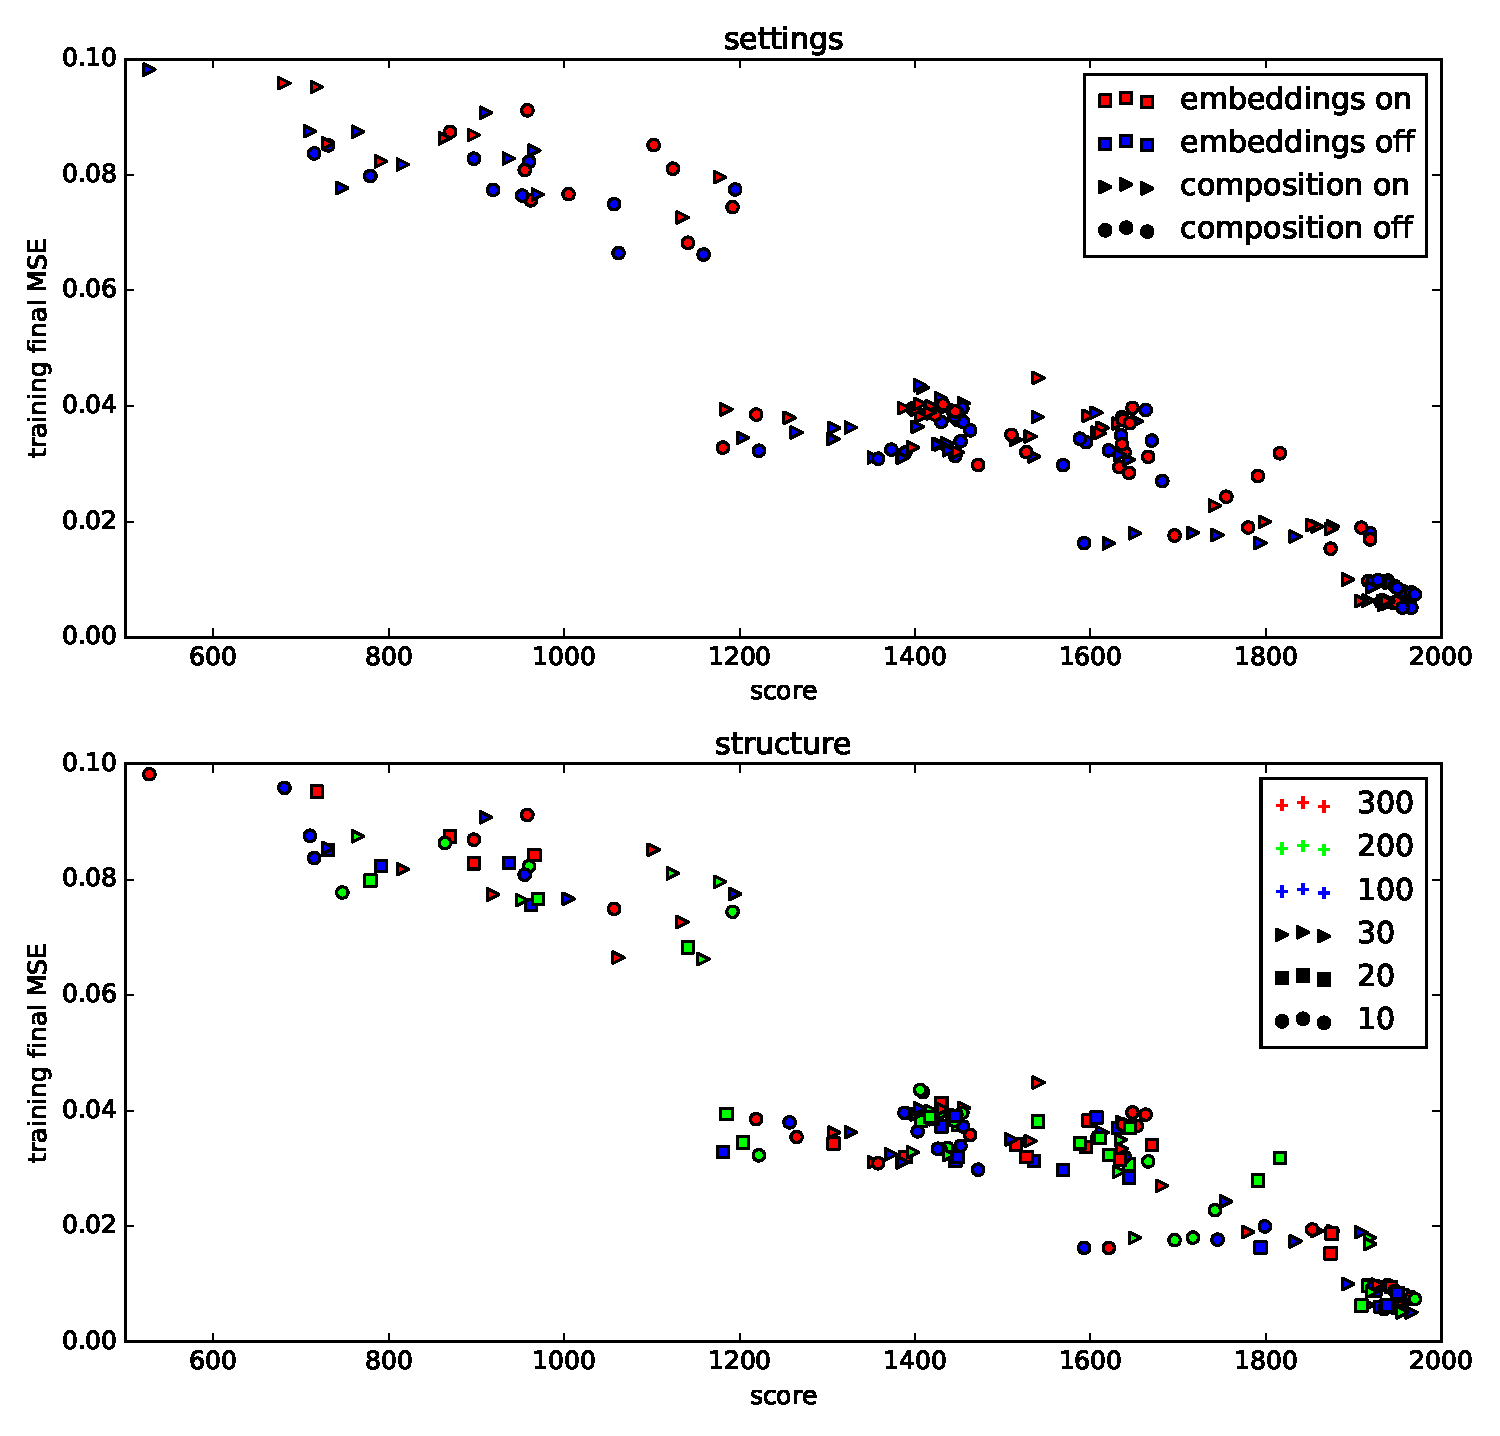
\includegraphics[width=\linewidth]{ext/figure_simples_cmb.pdf}
\caption{The plot shows results on a dataset containing only a simple shapes, without embeddings or conglomeration. Each point represents a single network. The x-axis shows achieved score according to the rules \ref{rules}, and the y-axis shows the achieved MSE of the network during training.
The first graph shows by color whether was trained to recognize embeddings, and by shape whether the network was trained to recognize conglomerations.
The second graph shows the structure of the network. The color marks the number of neurons in the first hidden layer and the shape marks the number of neurons in the second hidden layer.}
\label{fig:simples}
\end{figure}

\begin{figure}
\centering
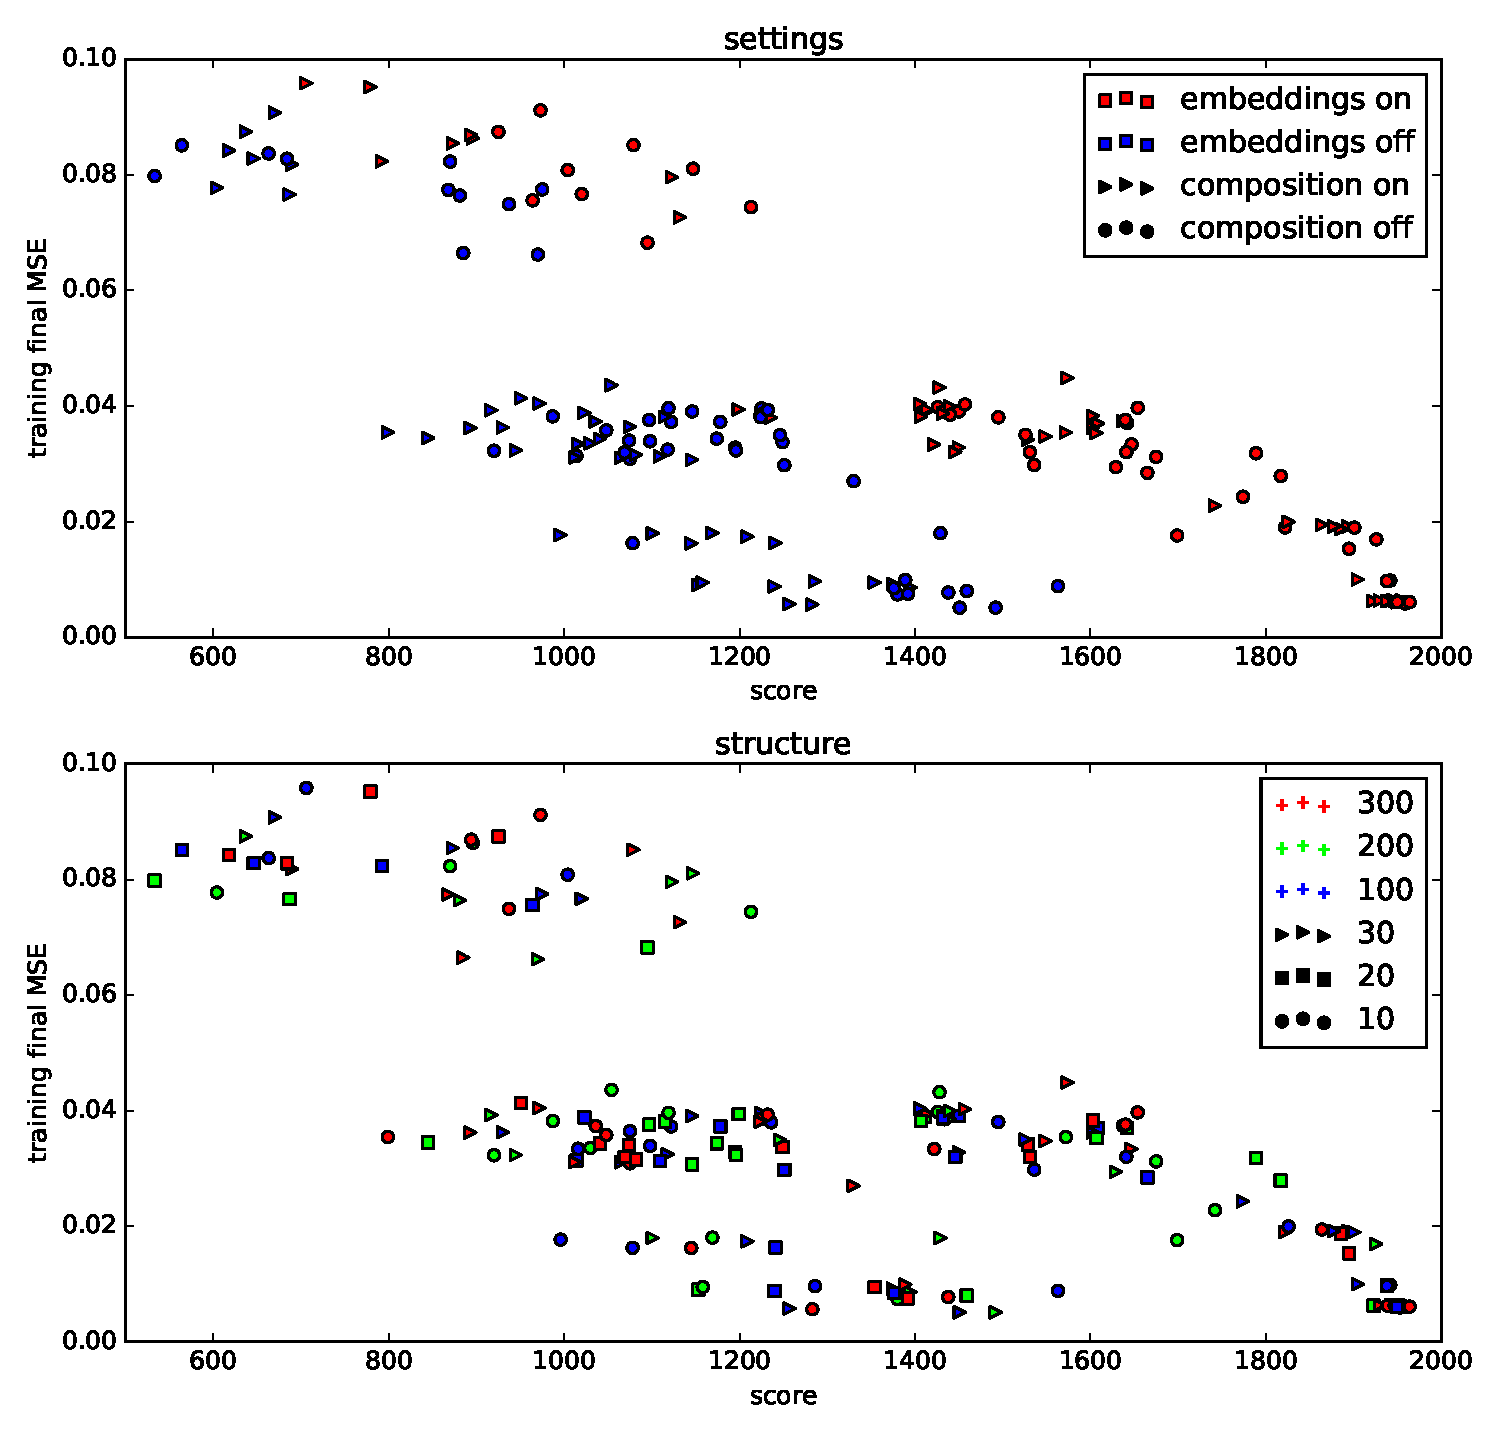
\includegraphics[width=\linewidth]{ext/figure_embed_cmb.pdf}
\caption{The plot shows result on a dataset containing embedded shapes. Each sample  contained shape with an embedded shape. For detailed information see figure \ref{fig:simples}.}
\label{fig:embed}
\end{figure}

\begin{figure}
\centering
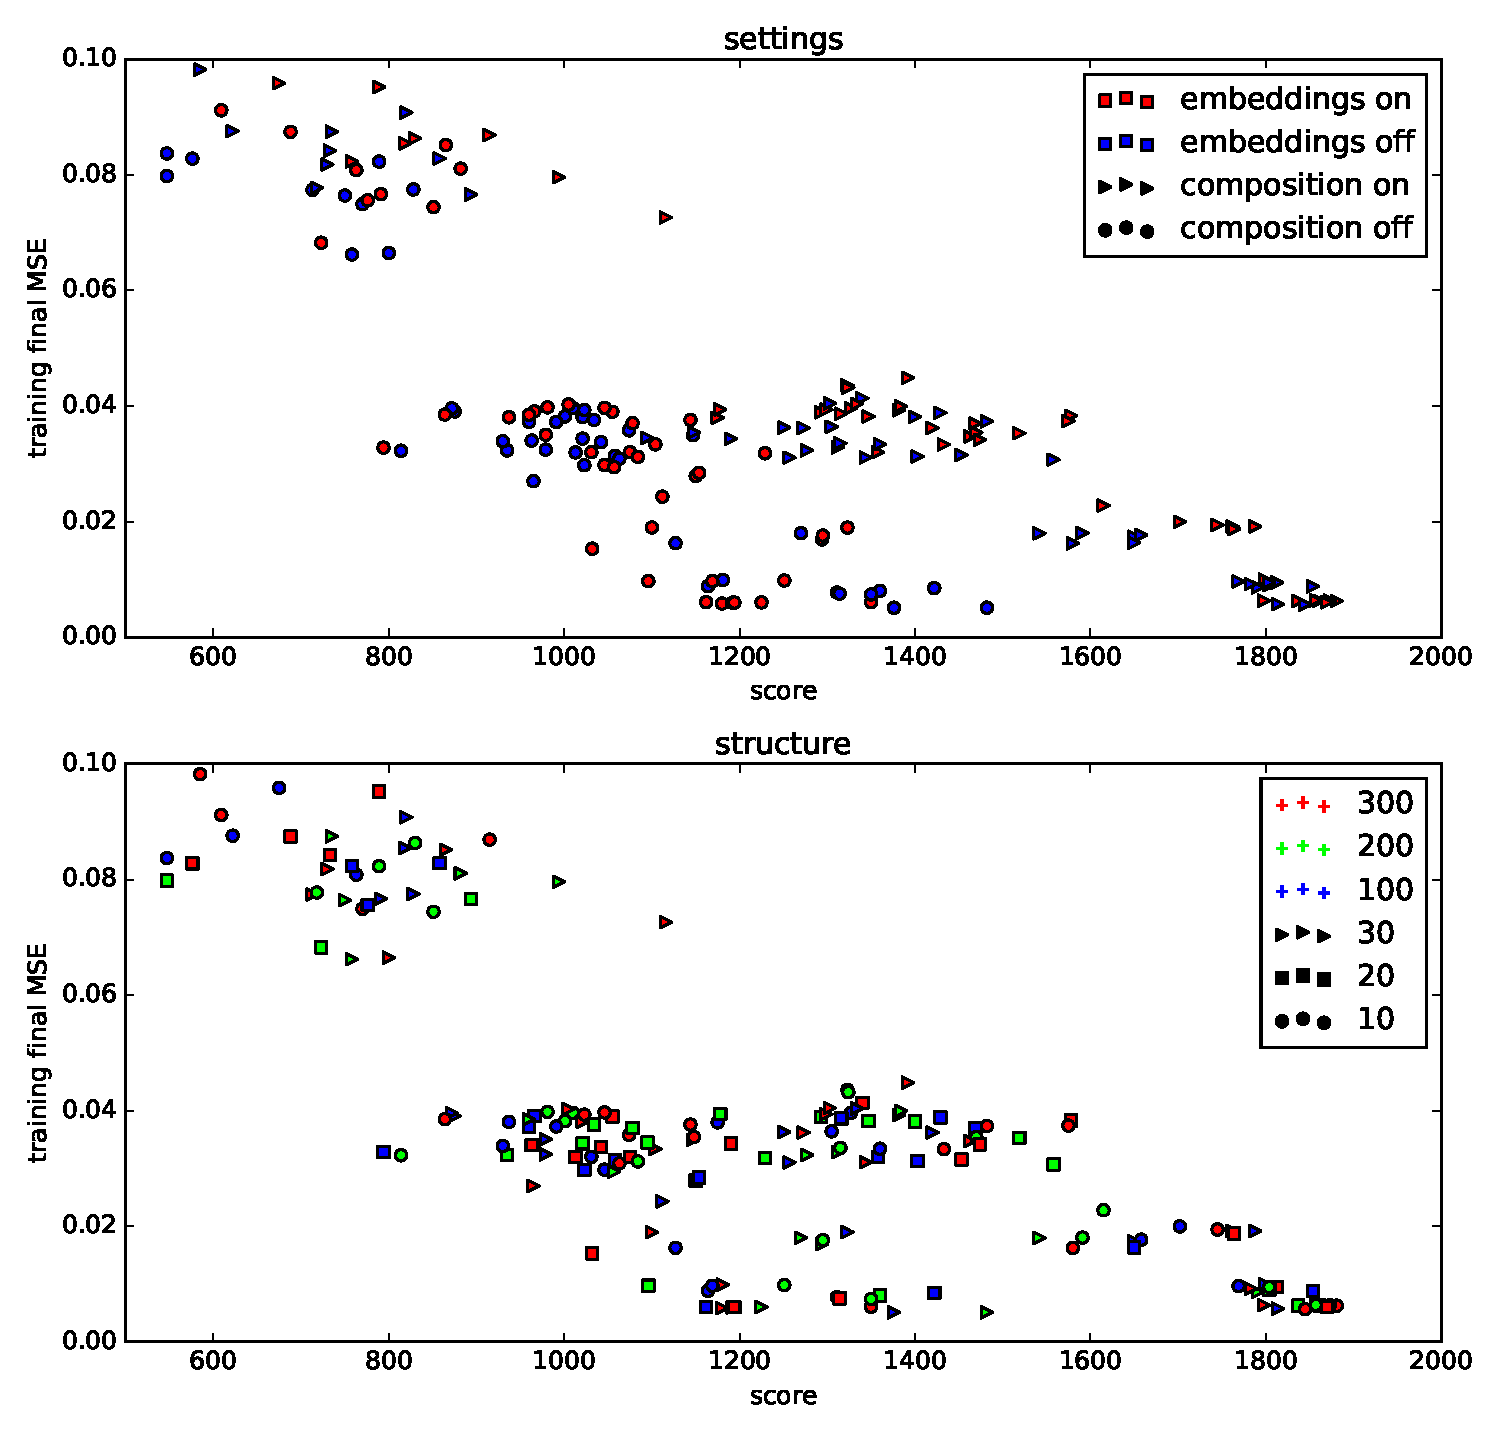
\includegraphics[width=\linewidth]{ext/figure_comp_cmb.pdf}
\caption{The plot shows result on a dataset containing composition of shapes. Each sample  contained shape composed from a number of instances of a pattern shape. For detailed information see figure \ref{fig:simples}.}
\label{fig:comp}
\end{figure}

\begin{figure}
\centering
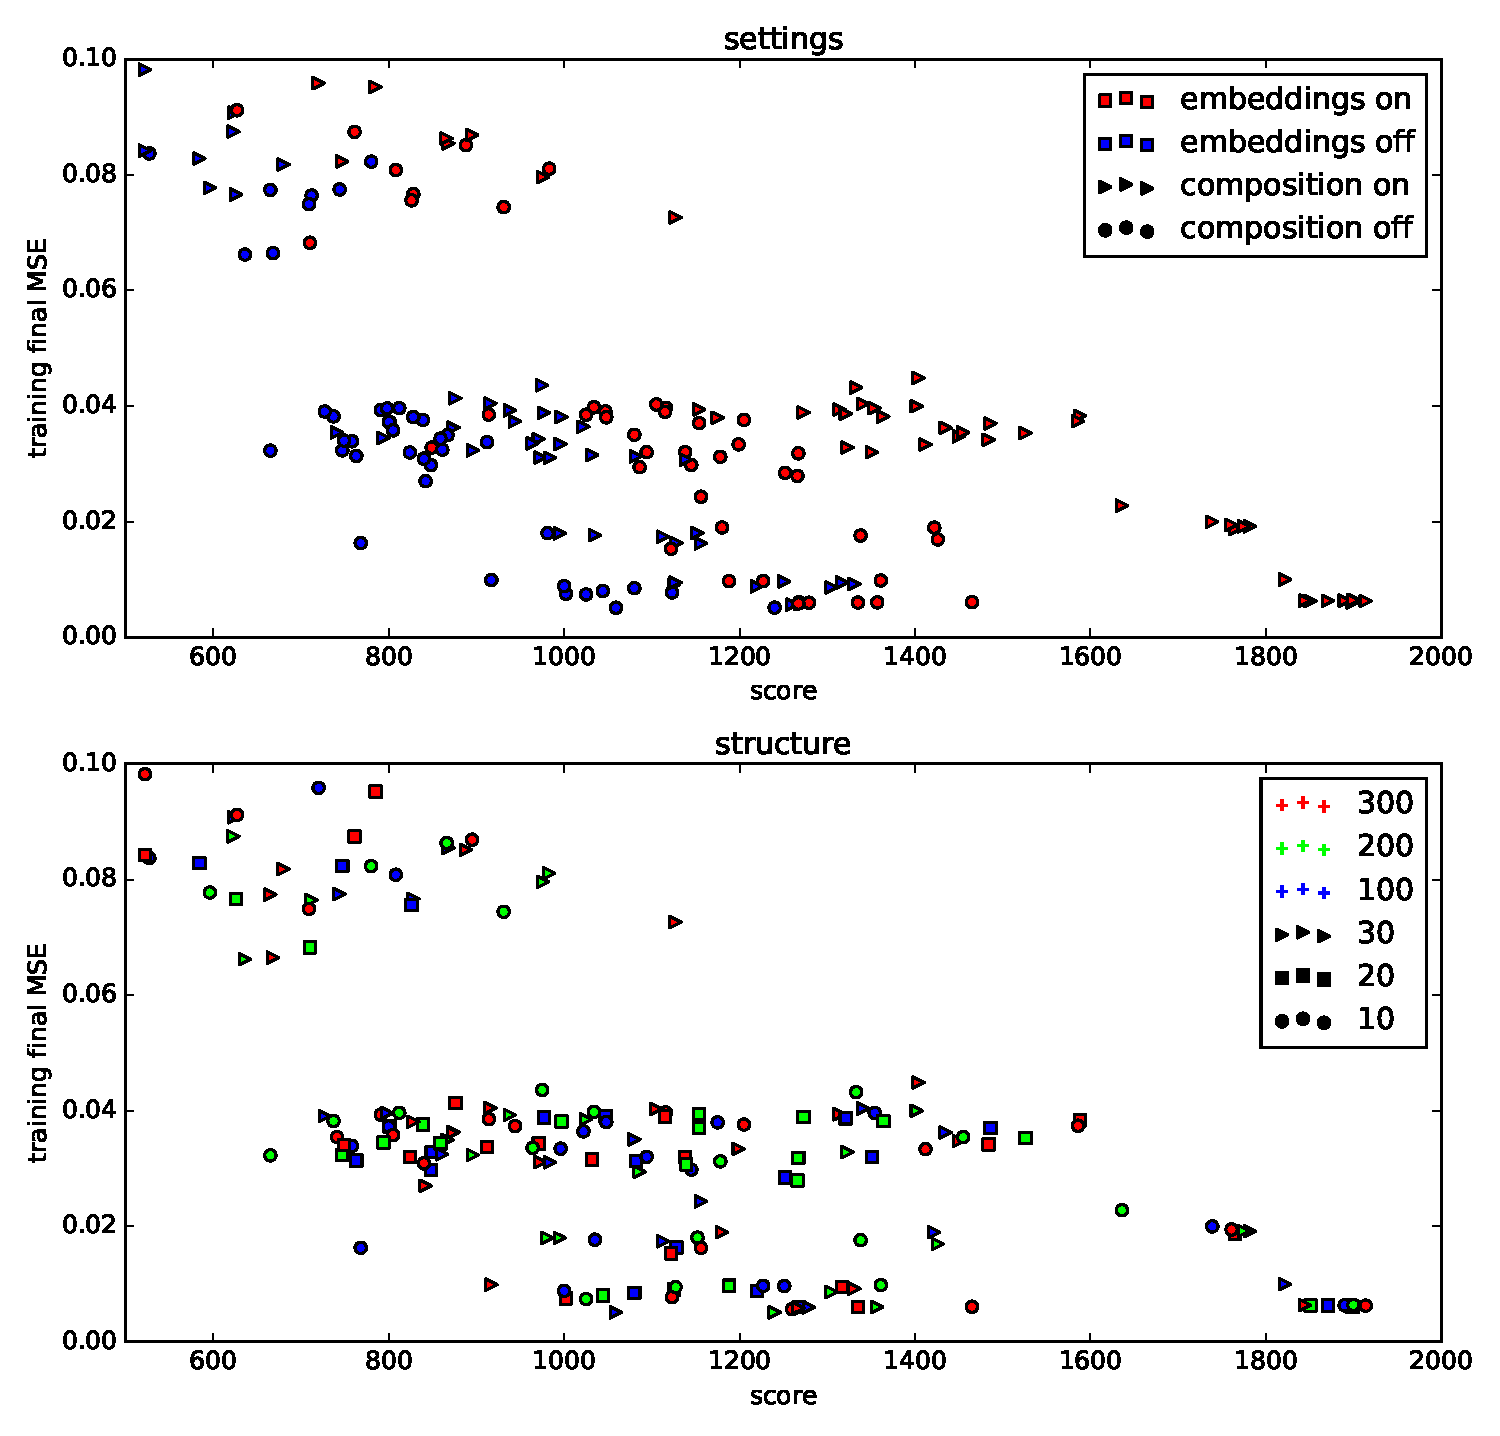
\includegraphics[width=\linewidth]{ext/figure_x_cmb.pdf}
\caption{The plot shows result on a dataset containing combination of embedded and composed shapes. Each sample contained a shape composed from a number of instances of a pattern shape and with an embedded shape. For detailed information see figure \ref{fig:simples}.}
\label{fig:cmb}
\end{figure}

There is a visible gap on the y-axis between 0.07 and 0.04 in all graphs. This is caused by the a sudden improvement when the network was trained to reach MSE under 0.07. It usually improved a lot more than that, finishing the training with a MSE around 0.04 or lower.

Another thing common among the graphs is that the figures plotting the influence of the structure do not show any clear pattern. All the layer sizes used in the tests were able to achieve good results, even the network with the lowest number of neurons. It may be necessary to increase the number for a higher count of shape descriptors, but for the four used shape descriptors, even the network with 100 neurons in first and 10 neurons in second layer was sufficient.

It can also be observed from the figures that the tendency to overtrain is not present even with very low MSE. It is then preferable to aim for a lower MSE values during training, as they clearly improve the achieved score.

However, one of the key results, visible in \cref{fig:simples}, is that training the network to recognize the embeddings and composition effects decreases the performance on the simple shapes only slightly if the network is trained with a low final MSE.

\section{Algorithm parameters optimization}
In this section, we test and evaluate the algorithm performance. In the evaluation, we use the best network trained for both embeddings and composition, since it was observed from the results, that network trained for both cases performs almost as well as networks trained for only one case. We try to optimize the algorithm parameters for the recognition of the used shape descriptors: square, circle, triangle and water drop. It may be possible that the parameters would have different optimal value for different shape descriptors. 

\todo{rference do apendixu kvuli vysvetleni parametru, nebo vytvorit vysveleni v imlpementaci?}
\subsection{Composition recognition}
To measure composition precision, we have prepared 100 \texttt{ImageLines} instances of composition examples. Each instance represents a shape composed of instances of another shape. We have also setup the algorithm this way:
\begin{enumerate}
\item \texttt{COMPOSED\_SHAPES\_ENABLED = true;}
\item \texttt{EMBEDDED\_SHAPES\_ENABLED = false;}
\item \texttt{ROTATION\_ENABLED = false;}
\end{enumerate}
This means that he algorithm searches for the pattern shape of the possible composition, but ignores embeddings locations and does not try different rotations.

We have tested different combinations of settings of these variables:
\begin{enumerate}
\item \texttt{COMPOSITION\_SAMPLES\_COUNT}
\item \texttt{COMPOSITION\_SAMPLES\_LIMIT}
\item \texttt{COMPOSITION\_WINDOW\_SIZE} 
\end{enumerate}

For each test instance we have compared the correct pattern shape with the recognized pattern shape.
In the results \ref{fig:com}, we can see that the success rate grows with the increasing number of samples. The algorithm has more chances to hit the area with the shape, rather than the area between the shapes and generally the chance to recognize at least one pattern shape is higher.

We can also see that the red and black colors representing the smaller sizes of the sample window perform better with the higher sample count, while being faster at the same time. The performance improvement for the smaller sample window tells us that the network does not recognize the shapes if the surrounding of the area covered by parts of other shapes. The speed improvement is caused by our line drawing algorithm. When the window size is smaller, there are fewer lines to draw per sample.

There is also a great drop in success rate when increasing the sample limit to more than one. This means that the network has trouble recognizing even a single pattern shape from the shapes that form conglomeration. There are two factors that affect the recognition of the pattern shape:
\begin{description} 
\item The sampling window follows the ideal path from the shape descriptor, but the real shape is usually more or less deformed, which means that the window will hit only a part of the pattern shape. 
\item The pattern shapes can be of various sizes which is hard to approximate by a single size of the sampling window. And if even the window hits the whole pattern shape, there is a very high chance of hitting also the noise from other shape patterns, or from embeddings.
\end{description}
Both factors make the recognition for the network very difficult. The network is rarely able to recognize even a single pattern shape correctly, and after 40 samples, the success rate does not improve much and stays somewhere between 40\% and 60\%.

It is clear that the algorithm becomes gradually slower with the increasing number of samples. The total time will also increase substantially if the rotation is turned on, because each composition sample is tested for all rotations.

\begin{figure}
\centering
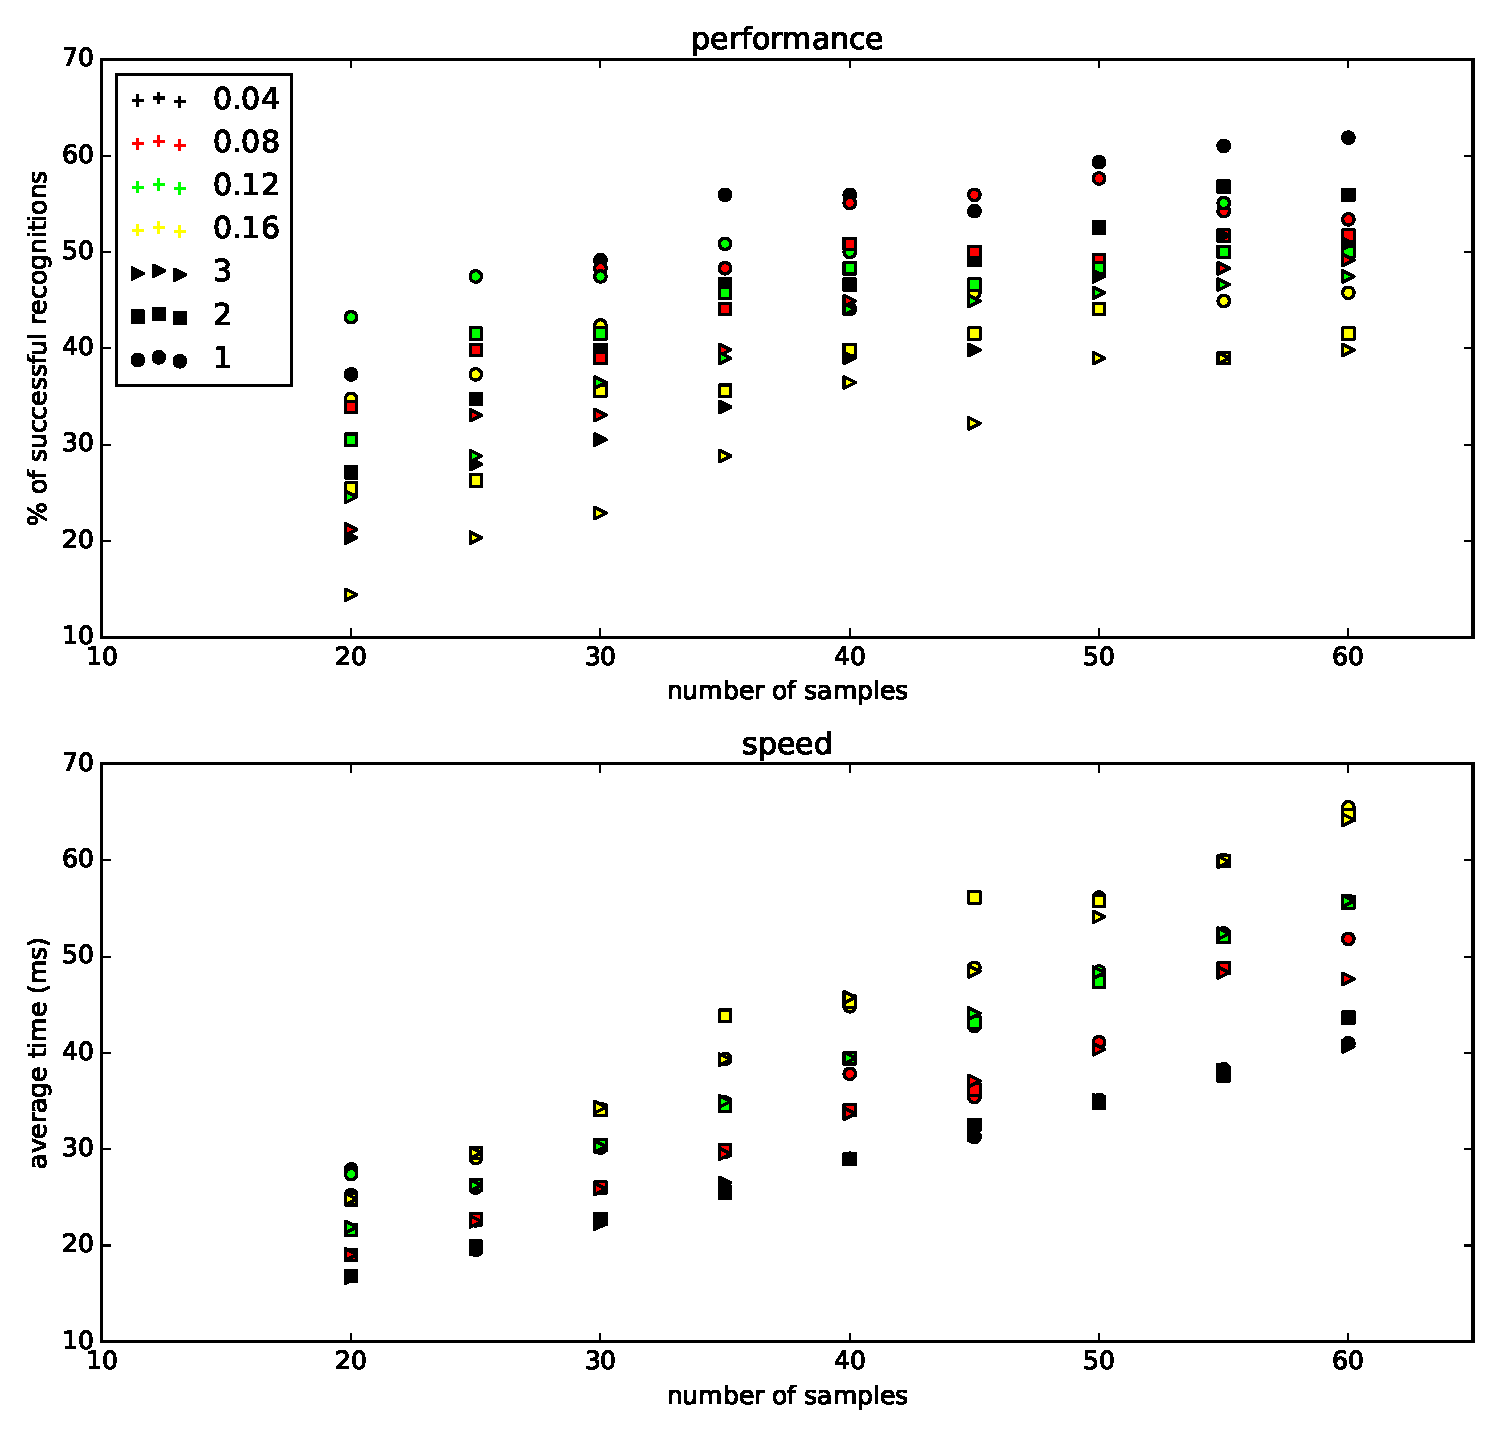
\includegraphics[width=.8\linewidth]{ext/figure_composition_results.pdf}
\caption{The x-axis shows the values of \texttt{COMPOSITION\_SAMPLES\_COUNT}, which is actually a count of samples made around the shape contour. The point color denotes the \texttt{COMPOSITION\_WINDOW\_SIZE}, and the point shape denotes the \texttt{COMPOSITION\_SAMPLES\_LIMIT} according to the legend. Each object of the plot then represents a combination of parameters settings and the performance and speed achieved with the parameters over the test samples. The y-axis of the first plot shows the successful recognitions percentage over the test samples, and in the second plot, the y-axis shows an average computation time per one sample.}
\label{fig:com}
\end{figure}

\section{Rotation}
Rotation invariance is achieved by redrawing the image at different angles and returning the best match from the rotated samples. We tested the influence of the \texttt{ROTATION\_SAMPLES\_COUNT} variable on the precision and speed of the algorithm. 

In the results \cref{fig:rotation} we can see that the precision of simple data shapes reaches almost 100\% at 15 samples. However, the recognition of the composed shapes is much worse. At 15 samples, it reaches about 70\% success rate and barely improves for the higher sample values. At the same time we know from \cref{fig:cmb} that the network is able to recognize composed shapes quite successfully. 

From these facts, we conclude that the problem are false matches of different shapes. A square composed from circles can at 45 degrees rotation closely resemble circle, and the network assigns the circle a higher match value than the square at the correct rotation. \todo{picture}

We can also observe from \cref{fig:rotation}, that the speed of the recognition of composed shapes is much slower and the gap is increasing with samples count. This is caused by the fact, that composed shapes contain a lot more lines than the simple shapes and each of these lines adds to the transformation time and to the drawing time.

We can deduce that setting ROTATION\_SAMPLES\_COUNT to higher than 15 is rather impractical.

\begin{figure}
\centering
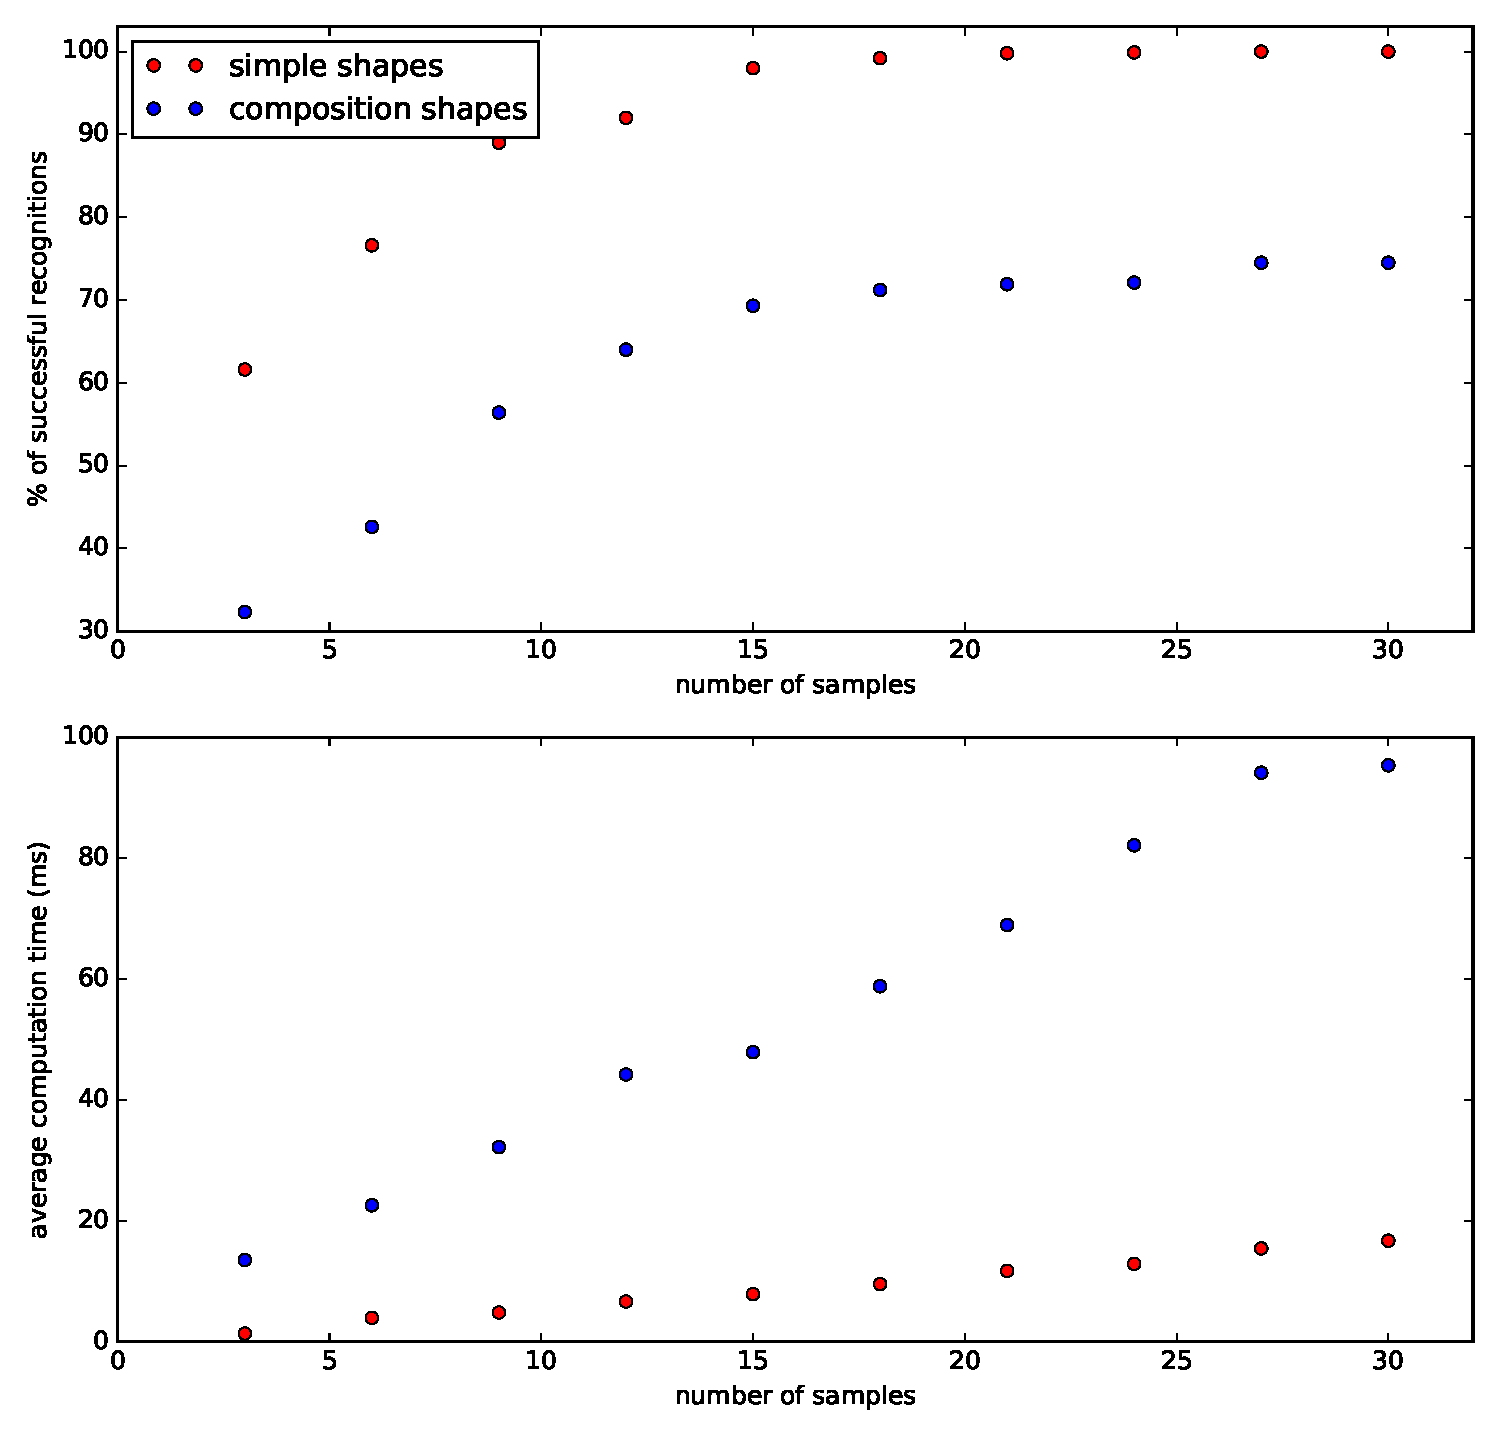
\includegraphics[width=\linewidth]{ext/rotation_cmb.pdf}
\caption{The x-axis shows the values of \texttt{ROTATION\_SAMPLES\_COUNT}. Each dot represents a test run over the test data. The red dots represent results over the test data with simple shapes, and the blue dots represent results over the test data with composed shapes. The y-axis of the first plot shows success recognition rate and in the second plot the y-axis shows an average computation time per one sample.}
\label{fig:rotation}
\end{figure}


\section{Embeddings}
The ability of the algorithm to recognize embeddings depends on the shape descriptor definition rather than on the algorithm settings. 

The user can define the points of interest by their position and size and these two parameters form a rectangular area where the algorithm will search for embedded shape. 

It is then recommended to set the size of this area lower, to avoid fragments of the top shape appearing in this area, which might cause the network to not recognize the embedded shape. If the embeddings are supposed to appear inside composed shapes, the area should be even smaller, otherwise, the fragments of the pattern shapes will appear inside. 

The speed influence of embeddings has a clear form. Every point of interest is analyzed and if the embedded shape is found, the algorithm runs recursively on the area of the embedded shape.

\todo{Chces sem dat nekolik screenshotu ze hry ktery demonstrujou jak to nakonec vypada. Zaroven by nebylo spatny ukazat nejakej malej sample tech trenovacich a generovanejch dat, pripadne nejaky outliery (ty sou vzdycky zajimavy). Obecne by hodne prospel i zajimavej obrazek toho co presne vizualne znamena embedding a composition, hned k zacatku tyhle kapitoly.}
